%!TEX root = egpaper_for_review.tex
\begin{figure}[H]

\tikzfading[name=fade right0,left color=transparent!0, right color=transparent!70]
\tikzfading[name=fade right1,left color=transparent!70, right color=transparent!100]
\tikzstyle{gNode}=[fill=white,draw,solid,font=\sffamily\small]
\tikzstyle{cutNode}=[fill=white,draw,solid,font=\sffamily\small]
\tikzstyle{opBox}=[fill=black,text=white,draw,solid,font=\sffamily\tiny,align=center]
\tikzstyle{label}=[fill=black,text=white,draw,solid,font=\sffamily\tiny]
\tikzstyle{edgeLabelNode}=[ellipse,text=black,solid,font=\sffamily\tiny,align=left,minimum size=0.5cm]
\tikzstyle{aEdge}=[->,node distance=0.5cm]
\begin{tikzpicture}
    
    \draw node[opBox] (gen) {GENERATOR};
    \draw node[cutNode,right = 1cm of gen] (proposal_cut) {$\bar{P}$};
    \draw node[right of = proposal_cut](dummy){};
    \draw node[cutNode,right of = dummy] (best_cut) {$P$};
    \draw node[opBox,below of = dummy] (intersect) {INTERSECT\\UNCUT};
    \draw node[cutNode,below of = intersect] (int_cut){$\tilde{P}$};
    \draw node[opBox,below of = int_cut] (contract) {CONTRACT\\UNCUT\\EDGES};
    \draw node[gNode,right = 2cm of contract](cgraph)  {$( \tilde{\mathcal{G}}, \tilde{\mathcal{W}})$};
    \draw node[opBox, above of =  cgraph] (multicut) {MULTICUT};
    \draw node[cutNode,above of = multicut] (rcut) {$\bar{P}^{\tilde{\mathcal{G}}}$};
    \draw node[opBox, above of =  rcut] (pback) {PROJECT\\CUT\\BACK};

    \node[draw,dotted,fit=(proposal_cut) (cgraph),inner sep = 3mm,thick, draw=gray,opacity=0.5] {};

    \draw node[gNode,below = of gen](graph)  {$( \mathcal{G}, \mathcal{W})$};
    \path[]
    (gen) edge[aEdge]  node[]{} (proposal_cut)
    (graph) edge[aEdge] (gen)
    (proposal_cut)  edge[aEdge]   (intersect)
    (best_cut)      edge[aEdge]   (intersect)
    (intersect)     edge[aEdge]   (int_cut)
    (int_cut)       edge[aEdge]   (contract) 
    (contract)      edge[aEdge,above]   
        node[edgeLabelNode]{coarse graphs\\with fewer nodes}(cgraph)
    (cgraph)        edge[aEdge]   (multicut)
    (multicut)      edge[aEdge]   (rcut)
    (rcut)          edge[aEdge]   (pback)
    (pback)         edge[aEdge]   (best_cut)
    (graph)         edge[aEdge]   (contract.west)
    (best_cut)      edge[aEdge,dashed,bend angle=90,bend right,draw=gray!30]  
        node[edgeLabelNode]{current best solution\\can influence generator}  (gen)
    ;
\end{tikzpicture}
\caption{
    The proposed algorithm works in the following way:
    Given a graph $\mathcal{G}$, edge weights $\mathcal{W}$ and
    a proposal generator, the current best solution $P$ is iteratively improved.
    A proposal generator generates different versatile
    proposal partitions $\bar{P}$.
    The proposal  $\bar{P}$ is intersected with $P$ which results in
    $\tilde{P}$. Contracting each each which is not 
    cut in $\tilde{P}$ leads to a coarser graph  
    $\tilde{\mathcal{G}} = ( \tilde{\mathcal{V}}, \tilde{\mathcal{E}} )$ 
    with new edge weights $\tilde{\mathcal{W}}$.
    If  $\bar{P}$ and $P$ have a small fraction of cut edges, $\tilde{\mathcal{G}}$ will be small ( $|\tilde{\mathcal{V}}| << |\mathcal{V}|$
    and $|\tilde{\mathcal{E}}| << |\mathcal{E}|$).
    The multicut objective on the smaller graph $\tilde{\mathcal{G}}$ can be optimized magnitudes 
    faster than on $\tilde{\mathcal{G}}$.
    It is guaranteed that the optimal multicut partitioning $\bar{P}^{\tilde{\mathcal{G}}}$ on $\tilde{\mathcal{G}}$ projected 
    back to $\mathcal{G}$ as a lower or equal energy than any of the two input partitions $P$ and $\bar{P}$, 
    therefore we store the result of fusion as new best state $P$ and repeat the procedure.
}\label{fig:algo_graph}
\end{figure}


\begin{figure}[H]

%\begin{tikzpicture}
%    \tikzstyle{pixel}=[regular polygon,regular polygon sides=4,inner sep=0pt,draw,solid,font=\sffamily\small]
%
%    \node[anchor=south west,inner sep=0] (image) at (0,0) {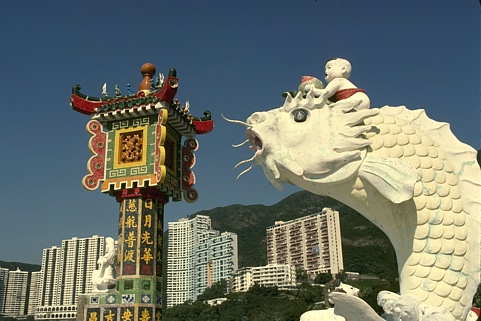
\includegraphics[width=.25\textwidth]{images/120093.jpg}};
%    \begin{scope}[x={(image.south east)},y={(image.north west)}]
%        \draw[red,ultra thick,rounded corners] (0.62,0.65) rectangle (0.78,0.75);
%        \draw node[pixel ](100.5,100.5) {BLAAA};
%    \end{scope}
%\end{tikzpicture}

% 481 / 321
\begin{tikzpicture}[scale=1.0]


    \node[anchor=south west,inner sep=0] (image) at (0,0) 
        {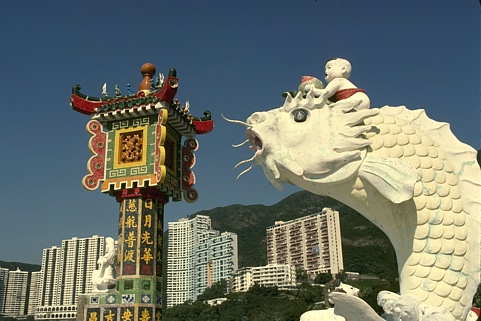
\includegraphics[width=.25\textwidth]{images/120093.jpg}};
    \begin{scope}[x={(image.south east)},y={(image.north west)},xscale=100/481,yscale=100/321]   
        %   \draw (0,0) grid (481,321);
        \draw[gray,xstep=3.21/15, ystep=3.21/15] (0,0) grid (4.81,3.21);
    \end{scope}


\end{tikzpicture}


\end{figure}
